%%%%%%%%%%%%%%%%%%%%%%%%%%%%%%%%%%%%%%%%%%%%%%%%%%%%%%%%%%%%%%%%%%%%%%
% Overleaf (WriteLaTeX) Example: Molecular Chemistry Presentation
%
% Source: http://www.overleaf.com
%
% In these slides we show how Overleaf can be used with standard 
% chemistry packages to easily create professional presentations.
% 
% Feel free to distribute this example, but please keep the referral
% to overleaf.com
% 
%%%%%%%%%%%%%%%%%%%%%%%%%%%%%%%%%%%%%%%%%%%%%%%%%%%%%%%%%%%%%%%%%%%%%%
% How to use Overleaf: 
%
% You edit the source code here on the left, and the preview on the
% right shows you the result within a few seconds.
%
% Bookmark this page and share the URL with your co-authors. They can
% edit at the same time!
%
% You can upload figures, bibliographies, custom classes and
% styles using the files menu.
%
% If you're new to LaTeX, the wikibook is a great place to start:
% http://en.wikibooks.org/wiki/LaTeX
%
%%%%%%%%%%%%%%%%%%%%%%%%%%%%%%%%%%%%%%%%%%%%%%%%%%%%%%%%%%%%%%%%%%%%%%

\documentclass{beamer}

% For more themes, color themes and font themes, see:
% http://deic.uab.es/~iblanes/beamer_gallery/index_by_theme.html
%
\mode<presentation>
{
  \usetheme{AnnArbor}       % or try default, Darmstadt, Warsaw, ...
  \usecolortheme{crane} % or try albatross, beaver, crane, ...
  \usefonttheme{serif}    % or try default, structurebold, ...
  \setbeamertemplate{navigation symbols}{}
  \setbeamertemplate{caption}[numbered]
} 

\usepackage[english]{babel}
\usepackage[utf8x]{inputenc}
\usepackage{chemfig}
\usepackage[version=3]{mhchem}

% On Overleaf, these lines give you sharper preview images.
% You might want to `comment them out before you export, though.
\usepackage{pgfpages}
\pgfpagesuselayout{resize to}[%
  physical paper width=8in, physical paper height=6in]


\title{Value Of Local Showrooms To Online Competitors}
% Here's where the presentation starts, with the info for the title slide
\author{\textbf{Author}: Jayarajan Samuel, Zhiqiang (Eric) Zheng, Ying Xie \\ 
{\footnotesize \textbf{Group Members}: Luoying Chen, Beyza Celik, Duc Vu, Yihong Liu }}
%\institute{www.overleaf.com}
\date{\today}

\begin{document}

\begin{frame}
  \titlepage
\end{frame}

% These three lines create an automatically generated table of contents.
\section{Advanced method}

\begin{frame}{Propensity Score Matching}
\begin{itemize}
  \item Nearest propensity score matching is used to match each zipcode from treatment group with an equivalent control group, using zip code level demographics. 
  \begin{itemize}
      \item Household size
      \item Household oldest age
      \item Household income
      \item Number of children
      \item Internet speed
  \end{itemize}
  \item After matching, we have left with 89 matched zip codes. Below are the propensity score before and after matching.
 \end{itemize}
\end{frame}

\begin{frame}{Propensity Score Matching}
\begin{figure}
     \centering
     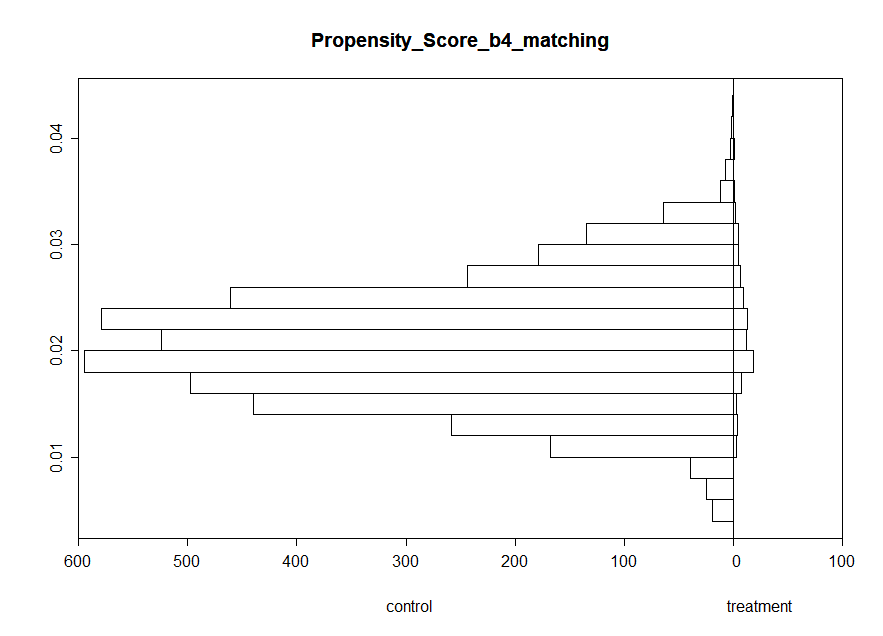
\includegraphics[width=\textwidth]{b4matching.png}
\end{figure}
\end{frame}

\begin{frame}{Propensity Score Matching}
\begin{figure}
     \centering
     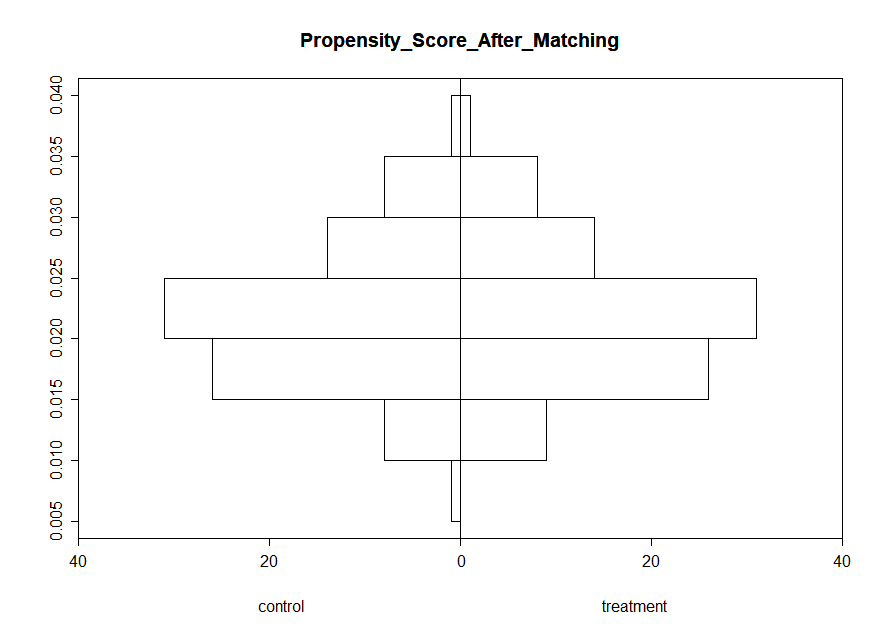
\includegraphics[width=\textwidth]{Aftermatching.png}
\end{figure}
\end{frame}

\begin{frame}{Propensity Score Matching}
\begin{table}[!htbp] \centering 
      \caption{Results of the Online Sales and Search Effect After Nearest Propensity Score Matching: TotalMonthlySales, PagesPerDollar, and MinsPerDollar (All Product Categories)} 
      \label{tab:tablepsm} 
      \resizebox{\columnwidth}{!}{
            \begin{tabular}{@{\extracolsep{1pt}}lD{.}{.}{-3} D{.}{.}{-3} D{.}{.}{-3} D{.}{.}{-3} D{.}{.}{-3} D{.}{.}{-3} } 
             \\[-1.8ex]\hline 
             \hline \\[-1.8ex] 
              % & \multicolumn{6}{c}{\textit{Dependent variable:}} \\ 
              %\cline{2-7} 
              %\\[-1.8ex]
              & \multicolumn{2}{c}{log(TotalMonthlySales + 1)} & \multicolumn{2}{c}{log(PagesPerDollar + 1)} & \multicolumn{2}{c}{log(MinsPerDollar + 1)} \\ 
              & \multicolumn{1}{c}{Amazon-0 Mile} & \multicolumn{1}{c}{BesyBuy-0 Mile} & \multicolumn{1}{c}{Amazon-0 Mile} & \multicolumn{1}{c}{BesyBuy-0 Mile} &                             \multicolumn{1}{c}{Amazon-0 Mile} & \multicolumn{1}{c}{BesyBuy-0 Mile} \\ 
              \\[-1.8ex] & \multicolumn{1}{c}{(1)} & \multicolumn{1}{c}{(2)} & \multicolumn{1}{c}{(3)} & \multicolumn{1}{c}{(4)} & \multicolumn{1}{c}{(5)} & \multicolumn{1}{c}               {(6)}\\ 
              \hline \\[-1.8ex] 
              $\beta_1$ & 0.029 & 0.0002 & 0.00004 & 0.0001 & 0.002 & 0.00000 \\ 
               & (0.024) & (0.031) & (0.020) & (0.009) & (0.019) & (0.005) \\ 
              $\beta_2$ & -0.033 & 0.009 & -0.068^{***} & 0.003 & -0.057^{***} & 0.0004 \\ 
              & (0.028) & (0.031) & (0.023) & (0.009) & (0.022) & (0.005) \\ 
              \hline \\[-1.8ex] 
              Observations & \multicolumn{1}{c}{3,000} & \multicolumn{1}{c}{768} & \multicolumn{1}{c}{3,000} & \multicolumn{1}{c}{768} & \multicolumn{1}{c}{3,000} &                           \multicolumn{1}{c}{768} \\ 
              R$^{2}$ & \multicolumn{1}{c}{0.001} & \multicolumn{1}{c}{0.001} & \multicolumn{1}{c}{0.004} & \multicolumn{1}{c}{0.001} & \multicolumn{1}{c}{0.003} &                           \multicolumn{1}{c}{0.00004} \\ 
              Adjusted R$^{2}$ & \multicolumn{1}{c}{-0.052} & \multicolumn{1}{c}{-0.078} & \multicolumn{1}{c}{-0.048} & \multicolumn{1}{c}{-0.078} & \multicolumn{1}{c}{-0.049}               & \multicolumn{1}{c}{-0.079} \\ 
              F Statistic & \multicolumn{1}{c}{0.935 (df = 2; 2850)} & \multicolumn{1}{c}{0.192 (df = 2; 711)} & \multicolumn{1}{c}{6.219$^{***}$ (df = 2; 2850)} &                           \multicolumn{1}{c}{0.185 (df = 2; 711)} & \multicolumn{1}{c}{4.693$^{***}$ (df = 2; 2850)} & \multicolumn{1}{c}{0.014 (df = 2; 711)} \\ 
              \hline 
              \hline \\[-1.8ex] 
              \textit{Note:}  & \multicolumn{6}{r}{$^{*}$p$<$0.1; $^{**}$p$<$0.05; $^{***}$p$<$0.01} \\ 
              \end{tabular}}
\end{table}
\end{frame}

\begin{frame}{Look-Ahead Propensity Score Matching}
\begin{itemize}
    \item LA-PSM requires some treated observations occur over different periods $t$ and $t+k$.
    \item Basic idea in LA-PSM is to match treated observations in period $t$ with observations which were in control group in period $t$ but in treatment group in period $t+k$.
    \item In this paper, Circuit City closed all their stores at the same time: November 2008.
    \item Therefore, LA-PSM method is not applicable.
\end{itemize}
\end{frame}

\end{document}
